\documentclass[10pt]{beamer}
\usepackage[english]{babel}
\setbeamertemplate{theorems}[numbered]
\setbeamertemplate{caption}[numbered]
\usefonttheme[onlymath]{serif}
\usetheme{Dallas}
\mode<presentation>
\setlength{\textwidth}{4.25in}
\parindent=0pt
\setlength{\parskip}{8pt}
\renewcommand{\baselinestretch}{1.0}

% Import graphics packages, set the graphics path
\usepackage{graphicx}
\graphicspath{{images/}}
\usepackage{subfig}
\usepackage{wrapfig}
\usepackage{multimedia}

\usepackage{changepage}

% Get rid of the navigation buttons
\setbeamertemplate{navigation symbols}{}

% % Add extra space under footnotes to make room for navigation buttons
% \addtobeamertemplate{footnote}{}{\vspace{2ex}}

% Import math packages
\usepackage{amssymb}
\usepackage{amsmath}
\usepackage{mathrsfs} % to use mathscr
\usepackage{dsfont}
\usepackage{physics}

% \usepackage[algo2e,ruled,vlined]{algorithm2e}
% \usepackage[]{algorithm2e}
\usepackage[ruled, vlined, linesnumbered, noend]{algorithm2e}
\usepackage{algorithmic}
\renewcommand{\algorithmicrequire}{\textbf{Input:}}
\renewcommand{\algorithmicensure}{\textbf{Output:}}
\usepackage{mathtools}

% Import packages for square, diamong, .. cirlces
\usepackage{fdsymbol}

% Define theorem-like environments


\SetKw{Return}{Return}
\SetKw{Find}{Find}
\SetKw{Define}{Define}

% Place the UTD logo in the frame titles
\usepackage{textpos}
\addtobeamertemplate{frametitle}{}{%
\begin{textblock*}{30mm}(.90\textwidth,-0.78cm)
% \includegraphics[height=0.7cm]{UT_Dallas_White.eps}
\end{textblock*}}
\addtobeamertemplate{frametitle}{}{%
\begin{textblock*}{30mm}(.73\textwidth,-0.75cm)
% \includegraphics[height=0.63cm]{conlab_logo_white_on_transparent.png}
% .73\textwidth: affects horizontal placement
% -0.75cm affects vertical placement
% [height=0.63cm] affects size of the image
\end{textblock*}}

% \begin{textblock*}{30mm}(.90\textwidth,-0.78cm)
% \includegraphics[height=0.7cm]{}
% \end{textblock*}

% Set the block styles
% Green
\setbeamercolor{block title}{use=structure,fg=white,bg=structure.fg}
\setbeamercolor{block body}{use=structure,fg=black,bg=structure.fg!3}
% Orange
% \setbeamercolor{block title}{use=structure,fg=white,bg=structure.bg}
% \setbeamercolor{block body}{use=structure,fg=black,bg=structure.bg!3}

% Navigation Stuff
\addtobeamertemplate{navigation symbols}{}{%
	\usebeamerfont{footline}%
	\usebeamercolor[fg]{footline}%
	\hspace{1em}%
	\insertframenumber/\inserttotalframenumber
}


% Set the itemize-like environment styles
\setbeamercolor{item}{fg=structure.fg,bg=structure.bg}
\setbeamertemplate{bibliography item}{\insertbiblabel}
\setbeamertemplate{itemize items}[square]
\setbeamertemplate{enumerate items}[square]

% Change the itemize-like environment spacings
\makeatletter
\def\@listI{\leftmargin\leftmargini
            \parsep 1pt
            \topsep 1pt
            \itemsep 1pt
            \parskip 2pt}
\makeatother

% Import definitions of command character sequences
%% Command definitions
% \def\i {\iota}
% mathbb
\def\bbb{\mathbb B}
\def\bbn{\mathbb N}
\def\bbz{\mathbb Z}
\def\bbq{\mathbb Q}
\def\bbr{\mathbb R}
\def\bbc{\mathbb C}
\def\bbs{\mathbb S}
\def\bbp{\mathbb P}
\def\bbe{\mathbb E}
%  mathbf
\def\bfx{\mathbf X}
\def\bfr{\mathbf R}
\def\bfs{\mathbf S}
% mathcal
\def\calx{\mathcal X}
\def\calu{\mathcal U}
\def\calr{\mathcal R}
\def\calp{\mathcal P}
\def\caln{\mathcal N}
\def\calf{\mathcal F}
\def\cali{\mathcal I}
\def\cald{\mathcal D}
\def\calo{\mathcal O}
\def\calc{\mathcal C}
\def\calt{\mathcal T}
\def\cals{\mathcal S}
% mathscr
\def\scrr{\mathscr R}
\def\scrp{\mathscr P}
\def\scrx{\mathscr X}
\def\scrt{\mathscr T}



%======== Abbreviations ==========================
\newcommand{\Max}{\max\limits_}
\newcommand{\Min}{\min\limits_}
\newcommand{\Sup}{\sup\limits_}
\newcommand{\Inf}{\inf\limits_}

\newcommand{\PP}{\mathbb{P}}
\newcommand{\EE}{\mathbb{E}}
\newcommand{\RR}{\mathbb{R}}
\newcommand{\XX}{\mathbb{X}}
\newcommand{\CC}{\mathbb{C}}
\newcommand{\BB}{\mathbb{B}}
\newcommand{\YY}{\mathbb{Y}}
\newcommand{\UU}{\mathbb{U}}
\newcommand{\NN}{\mathbb{N}}

\newcommand{\Ru}{\overline {\R}}
\newcommand{\Rl}{\underline {\R}}
\newcommand{\borel}{\mathfrak{B}}

\newcommand{\lra}{\longrightarrow}
\newcommand{\Lra}{\Longrightarrow}
\newcommand{\Lla}{\Longleftarrow}
\newcommand{\Llra}{\Longleftrightarrow}
\newcommand{\ra}{\rightarrow}
\newcommand{\da}{\downarrow}
\newcommand{\ua}{\uparrow}
\newcommand{\rra}{\rightrightarrows}
\newcommand{\ora}{\protect\overrightarrow}


\newcommand{\ind}{\mathds{1}}
\newcommand{\Let}{: =}
\newcommand{\teL}{= :}
\newcommand{\diff}{\mathrm{d}}
\newcommand{\mn}{\wedge}
\newcommand{\mx}{\vee}
\newcommand{\ol}[1]{\overline{#1}}
\newcommand{\wt}{\widetilde}
\newcommand{\wb}{\widebar}
\newcommand{\shift}{\vartheta}
\newcommand{\com}{\circ}
\newcommand{\tp}{\intercal}
\newcommand{\opt}{\star}
\newcommand{\ball}[2]{\mathsf{B}_{#2}(#1)}		%{\mathbb{B}\left(#1;#2\right)}
\newcommand{\ballC}{\overline{\mathsf{B}}}
\newcommand{\ballO}{\mathsf{B}}
\newcommand{\bigO}{\mathcal{O}}

\newcommand{\eqsmall}[1]{{\small $#1$}}
\newcommand{\goodgap}{\hspace{\subfigtopskip}}

\newcommand{\eps}{\varepsilon}
\DeclareMathOperator{\esup}{esssup}
\newcommand{\conv}{\mathsf{conv}}


\DeclareMathOperator{\vect}{vec}
% \DeclareMathOperator{\Tr}{Tr}

\DeclareMathOperator*{\argmax}{arg\,max}
\DeclareMathOperator*{\argmin}{arg\,min}

\newcommand{\RRT}{RRT}
\newcommand{\RRTs}{RRT*}
\newcommand{\ransrrt}{RANS-RRT*}


% Colors
\newcommand{\bbar}[1]{\bar{\bar{#1}}}
\renewcommand{\r}[1]{{\color{red}{#1}}}
\renewcommand{\b}[1]{{\color{blue}{#1}}}
\newcommand{\p}[1]{{\color{purple}{#1}}}
\newcommand{\g}[1]{{\color{OliveGreen}{#1}}}


%  Math 
\newcommand{\trnsp}[1]{{#1}^T}
\newcommand{\inv}[1]{{#1}^{-1}}
\newcommand{\invpar}[1]{\left ( {#1} \right) ^{-1}}
\newcommand{\invbrack}[1]{\left [ {#1} \right ] ^{-1}}

\newcommand{\absval}[1]{\mid {#1} \mid}
\newcommand{\innerprod}[1]{\langle {#1} \rangle}
% \newcommand{\norm}[1]{\left\lVert {#1} \right\rVert}
\newcommand{\rlbrack}[1]{\left [ {#1} \right]}
\newcommand{\rlbrace}[1]{\left \{ {#1}  \right\}}
\newcommand{\rlpar}[1]{\left ( {#1} \right)}

\newcommand{\matg}{\succ}
\newcommand{\matl}{\prec}
\newcommand{\matgeq}{\succeq}
\newcommand{\matleq}{\preceq}

\newcommand{\mean}[1]{\overline{{#1}}}
\newcommand{\expect}[1]{\bbe \rlbrack{{#1}}}



% Temporal Logic Operators
% Until
\newcommand{\until}[2]{\mathscr{U}_{[{#1},{#2}]}} % until with closed interval [a,b]
\newcommand{\untilI}[1]{\mathscr{U}_{{#1}}} % until with interval I
% Eventually
\newcommand{\finally}[2]{\mathscr{F}_{[{#1},{#2}]}} % eventually operator as F (finally) with closed interval [a,b]
\newcommand{\finallyI}[1]{\mathscr{F}_{#1}} % eventually operator as F (finally) with interval I
\newcommand{\eventually}[2]{\diamondsuit_{[{#1},{#2}]}} % eventually operator as a rhombus with closed interval [a,b]
% Always
\newcommand{\globally}[2]{\mathscr{G}_{[{#1},{#2}]}} % always operator as G (globally) with closed interval [a,b]
\newcommand{\globallyI}[1]{\mathscr{G}_{#1}} % always operator as G (finally) with interval I
\newcommand{\always}[2]{\square_{[{#1},{#2}]}} % always operator as a square with closed interval [a,b]

% Gaussian Distribution
\newcommand{\gaussd}[2]{\mathcal{N}\rlpar{{#1}, {#2}}} 


%======== Theorems and Definitions ==========================
% \newtheorem{lemma}{Lemma}
% \newtheorem{remark}{Remark}
% \newtheorem{prop}{Proposition}
% \newtheorem{theorem}{Theorem}
% \newtheorem{corollary}{Corollary}
% \newtheorem{conjecture}{Conjecture}
% \newtheorem{assump}{Assumption}
% \theoremstyle{definition}
% \newtheorem{example}{Example}
% \newtheorem{problem}{Problem}
% \newtheorem{definition}{Definition}


\newtheorem{lemmaN}{Lemma}
\newtheorem{remark}{Remark}
\newtheorem{prop}{Proposition \propnumber}
\newtheorem{theoremN}{Theorem}
\newtheorem{corollaryN}{Corollary}
\newtheorem{conjecture}{Conjecture}
\newtheorem{assump}{Assumption}
\theoremstyle{definition}
\newtheorem{examp}{Example}
\newtheorem{problemN}{Problem}
\newtheorem{definitionN}{Definition}

\newcommand{\propnumber}{} % initialize
\newenvironment{propc}[1]
  {\renewcommand{\propnumber}{#1}%
   \begin{prop}}
  {\end{prop}}
\newtheorem{exercise}{Exercise}


\DeclareMathOperator{\reshape}{reshape}
\DeclareMathOperator{\gare}{gare}

% Double underscore without spaces i.e. for writing Python __init__, __main__, etc.
\newlength\dunder
\settowidth{\dunder}{\_}
\newcommand{\twound}{\rule{2\dunder}{0.4pt}}

% Bold rich color
% Green
\def\bgr{\em\bf\color{UTDseafoam!75!UTDgreen}} % light green
\def\bdgr{\em\bf\color{UTDseafoam!50!UTDgreen}} % dark green
% Orange
\def\bor{\em\bf\color{UTDorange!50!orange}} % orange
% Math version of bor and bdgr
\def\mor{\color{UTDorange!50!UTDorange}} % orange
\def\mdgr{\color{UTDseafoam!50!UTDgreen}} % green
\def\mdsf{\color{UTDseafoam!50!UTDseafoam}} % seafoam






%Logo and Image Packages
\usepackage{graphicx}
\logo{
\includegraphics[width=1.5in]{Images/UT_Dallas_Logo}}

%Additional Packages
\usepackage{physics}
\usepackage{setspace}

%Presentation Info
\title[Network Analysis of FRC Matches]{Match Structures Changes as the FIRST Robotics Competition Program Evolved}
\subtitle{Network Analysis of FRC Matches}
\author{Jonas Wagner}
\institute[UTDallas]{Univeristy of Texas at Dallas}
\date[2021-05-07]{SYSM 6302 Final Project\\ 2021 May 7th}




% The whole document
\begin{document}
\begin{frame}
	\titlepage
\end{frame}

\section{Background on FRC Matches}
\begin{frame}{FIRST Robotics Competition}
	
\end{frame}

\begin{frame}{Current Event Match Structure}
	
\end{frame}

%------------------------------------------------------------
\section{Data Collection and Network Construction}
%------------------------------------------------------------
\begin{frame}{The Blue Alliance}
	content...
\end{frame}

%------------------------------------
\subsection{TBA\_Database\_Access.py}
%------------------------------------
\begin{frame}{Accessing The Blue Alliance Database}
	content...
\end{frame}

%-------------------------------------
\subsection{TBA\_Network\_Analysis.py}
%--------------------------------------
\begin{frame}{Network Generation}
	content...
\end{frame}

\begin{frame}{Network Methods}
	content...
\end{frame}

%--------------------------------------------------------
\section{Analysis Results}
%------------------------------------------------------
\subsection{Basic Analysis on Projections}
%----------------------------------------
\begin{frame}{2015 Hopper Sub-Division Analysis}
	\begin{columns}
		\column{0.5 \textwidth}
			testing\\
			s;ldfkaj
		\column{0.3 \textwidth}
			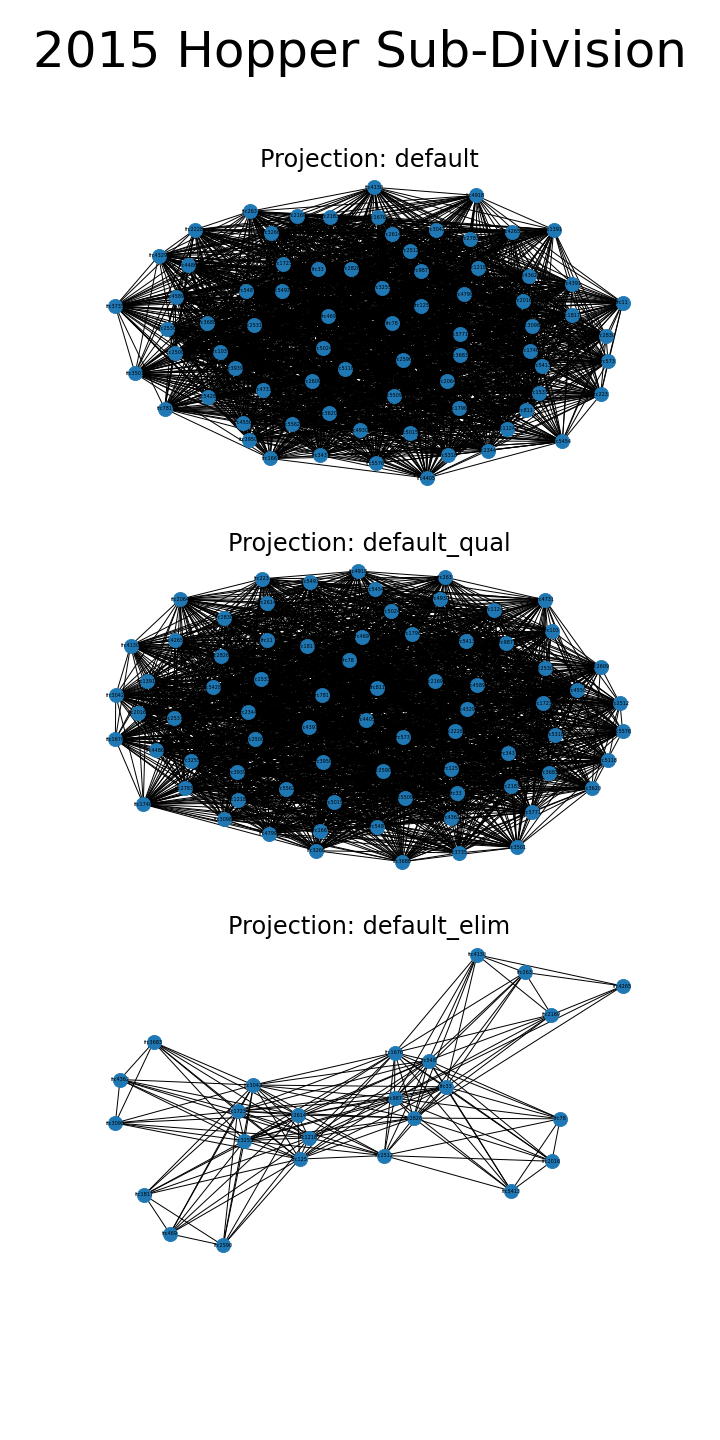
\includegraphics[height=\textheight]{../fig/NetworkPlot_2015hop}
	\end{columns}
\end{frame}




%\begin{frame}
	\titlepage
\end{frame}

\begin{frame}{Outline}
	\tableofcontents
\end{frame}
%% \begin{frame}
% \titlepage % Print the title page as the first slide
% \end{frame}

% \begin{frame}
% % \frametitle{Overview} % Table of contents slide, comment this block out to remove it
% \tableofcontents % Throughout your presentation, if you choose to use \section{} and \subsection{} commands, these will automatically be printed on this slide as an overview of your presentation
% \end{frame}

%----------------------------------------------------------------------------------------
%	PRESENTATION SLIDES
%----------------------------------------------------------------------------------------

%-------------------------------------------------------------
%%%%%%%%%%%%%%%%%%%%%%%%%%%%%%%%%%%%%%%%%%%%%%%%%%%%%%%%%%%%%%%%%%%%%%%
% \begin{frame}{~}
%     \begin{center}
%         \huge{Section Title}
%     \end{center}
% \end{frame}{}

% \begin{frame}{~}
%     \begin{center}
%         \LARGE{Subsection/algorithm title}
%     \end{center}
% \end{frame}{}

% \begin{frame}{Title}{}
%     Normal Text \\
%     \textbf{Bold Text}: definitions \\
%     \emph{emphasis text}: emphasizing key words \\
%     {\bor Orange text}: link to orange math \\
%     {\bdgr Dark green text}: link to dark green math \\
%     $ {\mor something}$: emphasize math term \\
%     $ {\mdgr something2}$: emphasize math term 
% \end{frame}{}

% \begin{frame}{Overview}{}
%     \begin{figure}[htb]
%         \centering
%         \includegraphics[width=0.5\columnwidth]{figures/placeholder.png}
%         \caption{caption}
%         \label{fig:f}
%     \end{figure}
% \end{frame}{}

% \begin{frame}{Overview}{}
%     \begin{columns}
%     \column{0.5\textwidth}
%         \begin{figure}[]
%             \centering
%             \includegraphics[trim=10cm 7cm 5cm 1cm, clip, width=1\columnwidth]{figures/placeholder.png} % left bottom right top
%             \caption{f1}
%             \label{fig:f1}
%         \end{figure}
%     \column{0.5\textwidth}
%         \begin{figure}[]
%             \centering
%             \includegraphics[width=1.\columnwidth]{figures/placeholder.png}
%             \caption{f2}
%             \label{fig:f2}
%         \end{figure}
%     \end{columns}
%     \url{https://url.com}
% \end{frame}{}


%%%%%%%%%%%%%%%%%%%%%%%%%%%%%%%%%%%%%%%%%%%%%%%%%%%%%%%%%%%%%%
% 1 Introduction
%%%%%%%%%%%%%%%%%%%%%%%%%%%%%%%%%%%%%%%%%%%%%%%%%%%%%%%%%%%%%%

\begin{frame}{Introduction}{\cite{vandenberghe2012convex,Soderstrom1988System}}

\textbf{System Identification}: Field of building mathematical models of dynamic systems from input and output signals.
\begin{itemize}
\item Large field: Can only cover a mere fraction of system identification here
\item This presentation focuses on system identification through {\bor low-dimensional model} structure creation
\end{itemize}
Typically, {\bor low-dimensional model} structure is expressed in {\bdgr low matrix rank} or {\bdgr sparsity of parameters}
\begin{itemize}
    \item Why {\bdgr matrix rank}: minimizing rank of model lowers the model dimension (\textbf{related to nuclear norm})
    \item Why {\bdgr sparsity of parameters}: maximizing sparsity will achieve the output with the fewest parameters (\textbf{related to 1-norm})
\end{itemize}
\end{frame}{}

%%%%%%%%%%%%%%%%%%%%%%%%%%%%%%%%%%%%%%%%%%%%%%%%%%%%%%%%%%%%%%
% 2 System Identification
%%%%%%%%%%%%%%%%%%%%%%%%%%%%%%%%%%%%%%%%%%%%%%%%%%%%%%%%%%%%%%

\begin{frame}{~}
    \begin{center}
        \huge{System Identification Problem}
    \end{center}
\end{frame}{}


\begin{frame}{System Identification}{1/2: Overview \ \ \cite{vandenberghe2012convex}}

%\begin{itemize} %List example on SVD?
% Pure \textbf{Singular Value Decomposition} works for low-rank approximation. However, the structure in the approximated matrices is tailored. \\
% \smallskip
{\bor Convex optimization} uses the nuclear norm to promote low rank while preserving linear matrix structure.\\
\smallskip
Consider the following structure where $Y$ and $U$ are \textbf{Hankel} matrices:
%\end{itemize}
{\scriptsize
\begin{align*}
    \begin{bmatrix}
        y(0) & y(1) & \hdots & y(N-1)\\
        y(1) & y(2) & \hdots & y(N)\\
        \vdots & \vdots & \ddots & \vdots\\
        y(s-1) & y(s) & \hdots & y(N+s-2)
    \end{bmatrix}
    = 
    {\mor \begin{bmatrix}
        C\\ CA\\ CA^2\\ \vdots\\ CA^{s-1}
    \end{bmatrix}}
    \begin{bmatrix}
        x(0) & x(1) & \hdots & x(N-1)
    \end{bmatrix} \\
    % 
    + 
    {\mdgr \begin{bmatrix}
        D & 0 & 0 & \hdots & 0\\
        CB & D & 0 & \hdots & 0\\
        CAB & CB & D & \hdots & 0\\
        \vdots & \vdots & \vdots & \ddots & \vdots\\
        CA^{s-2}B & CA^{s-3}B & \hdots & CB & D
    \end{bmatrix}}
    \begin{bmatrix}
        u(0) & u(1) & \hdots & u(N-1)\\
      u(1) & u(2) & \hdots & u(N)\\
      \vdots & \vdots & \ddots & \vdots\\
      u(s-1) & u(s) & \hdots & u(N+s-2)
    \end{bmatrix}
\end{align*}
}%
\begin{align*}
    Y = {\mor O}X + {\mdgr H}U
\end{align*}
% \begin{center}
% {\scriptsize \mqty[y(0) & y(1) & \hdots & y(N-1)\\
%       y(1) & y(2) & \hdots & y(N)\\
%       \vdots & \vdots & \ddots & \vdots\\
%       y(s-1) & y(s) & \hdots & y(N+s-2)] = \mqty[C\\ CA\\ CA^2\\ \vdots\\ CA^{s-1}]\mqty[x(0) & x(1) & \hdots & x(N-1)]\\
%       + \mqty[D & 0 & 0 & \hdots & 0\\
%       CB & D & 0 & \hdots & 0\\
%       CAB & CB & D & \hdots & 0\\
%       \vdots & \vdots & \vdots & \ddots & \vdots\\
%       CA^{s-2}B & CA^{s-3}B & \hdots & CB & D]\mqty[u(0) & u(1) & \hdots & u(N-1)\\
%       u(1) & u(2) & \hdots & u(N)\\
%       \vdots & \vdots & \ddots & \vdots\\
%       u(s-1) & u(s) & \hdots & u(N+s-2)]}
% \end{center}
    %   \newline
    %   \begin{center}
    %   \(Y = OX + HU\)
    %   \end{center}
\end{frame}{}

\begin{frame}{System Identification}{2/2: Process \ \  \cite{vandenberghe2012convex,Ljung1986System}}
Using \(Y = {\mor O}X + {\mdgr H}U\), the basis of the nullspace of $U$ can cancel terms.
\begin{align*}
    Q = I - U^T(UU^T)^{-1}U \quad \text{where} \quad UQ = U - UU^T(UU^T)^{-1}U = 0
\end{align*}
\begin{align*}
    YQ = {\mor O}XQ
\end{align*}
% \begin{center}
% \(Q = I - U^T(UU^T)^{-1}U \quad \text{where} \quad UQ = U - UU^T(UU^T)^{-1}U = 0\)\\
% \(YQ = OXQ\)
% \end{center}
Using this, the SDP below minimizes the rank of $YQ$ given the measurements $y_m(t)$ and inputs can be subject to noise. Here, $\lambda$ is a \textbf{weighting parameter} that has an inverse relationship with fitting error but matrix rank increases with increasing $\lambda$.
\begin{align*}
    \min \quad \norm{YQ}_* +\lambda\sum_{t=0}^{N}\norm{y(t) - y_m(t)}_2^2
\end{align*}
% \begin{center}
% \(\text{minimize } \norm{YQ}_* +\lambda\sum_{t=0}^{N}\norm{y(t) - y_m(t)}_2^2\) %Insert picture of results?
% \end{center}

General-purpose convex optimization solvers (e.g. CVX, YALMIP) can be used for \textbf{small} to \textbf{medium} sized problems. \textbf{Large} problems outside the scope of these solvers can be solved using algorithms presented in subsequent slides.
\end{frame}

% \begin{frame}{System Identification}{3/3: Aftermath}
% % Add what to do after you have solve the optimization problem.
% \small{To tie this section up with what to do after \(Y\) has been solved:}
% \begin{enumerate}
%     \item Compute the SVD: \(Y = U'\Sigma V^T\)
%     \item \(U'\) equates to \(OT\) =
%     $\begin{bmatrix}
%         CT\\ CT(T^{-1}AT)\\ \vdots\\ CT(T^{-1}AT)^{s-1}
%     \end{bmatrix}
%     = 
%     \begin{bmatrix}
%         \hat{C}\\ \hat{C}\hat{A}\\ \vdots \\ \hat{C}\hat{A}^{s-1}
%     \end{bmatrix}
%     $
%     % \mqty[CT\\ CT(T^{-1}AT)\\ \vdots\\ CT(T^{-1}AT)^{s-1}] = \(\mqty[\hat{C}\\ \hat{C}\hat{A}\\ \vdots \\ \hat{C}\hat{A}^{s-1}]\)
%     , where \(T\) is an unknown similarity transformation. \(\hat{C}\) can be extracted from the first block.
%     \item $\hat{A}$ can be computed from
%     $\begin{bmatrix}
%         \hat{C}\hat{A}\\ \vdots\\ \hat{C}\hat{A}^{s-1}
%     \end{bmatrix} = 
%     \begin{bmatrix}
%         \hat{C}\\ \vdots \\ \hat{C}\hat{A}^{s-2}
%     \end{bmatrix} \hat{A}$
%     % \(\mqty[\hat{C}\hat{A}\\ \vdots\\ \hat{C}\hat{A}^{s-1}] 
%     % = \mqty[\hat{C}\\ \vdots \\ \hat{C}\hat{A}^{s-2}]
%     % \hat{A}\)
%     \item Find \(\hat{B}, \hat{D},\) \& \(\hat{x}(0)\) from:
%     \(\hat{C}\hat{A}^t\hat{x}(0)+\sum_{k=0}^{t-1}\hat{C}\hat{A}^{t-k}\hat{B}u(k)+\hat{D}u(t) = y(t), t=0 \rightarrow N\)
%     \end{enumerate}
% More approximation techniques can be found in [INSERT REFERENCE].
% \end{frame}

%%%%%%%%%%%%%%%%%%%%%%%%%%%%%%%%%%%%%%%%%%%%%%%%%%%%%%%%%%%%%%
% 3 Graphical Models
%%%%%%%%%%%%%%%%%%%%%%%%%%%%%%%%%%%%%%%%%%%%%%%%%%%%%%%%%%%%%%

\begin{frame}{Graphical Models}{1/2: Overview \ \ \cite{vandenberghe2012convex}}
\begin{itemize}
    \item \textbf{Graphical models} are used for conditional dependence relations in optimal control (e.g. dynamic programming, markov processes)
    \item \(x \sim{~} \mathcal{N}(\mu,\Sigma)  \)
    \begin{itemize}
        \item The vertices are the components of \(x\)
        \item Vertices \(i\) and \(j\) are connected if there is a nonzero in the \(i,j\) position of the inverse covariance matrix \(\Sigma^{-1}\)
    \end{itemize}
    \item These graphs can be estimated through {\bor convex optimization}
\end{itemize}
\end{frame}


\begin{frame}{Graphical Models}{2/2: Process \ \ \cite{vandenberghe2012convex, ravikumar2008highdimensional}}
\begin{itemize}
    \item With n samples \(y\), the second moment matrix about the mean \(C\) is calculated:\\
    \begin{center}
        \(C = \frac{1}{n}\sum_{k=1}^{n}(y^{k}-\mu)(y^{k}-\mu)^T\)
    \end{center}
    \item From \textbf{Bregman divergence}, the estimate of the inverse covariance \(\Sigma^{-1}\) is obtained with:\\
    \begin{center}
        \( \max \quad \log\rlpar{det(\Sigma^{-1})} - \tr{C\Sigma^{-1}}-\lambda \norm{\Sigma^{-1}}_1\)\\
     \end{center}
        or\\
     \begin{center}
        \(\min \quad \tr{C\Sigma^{-1}} - log\rlpar{det(\Sigma^{-1})} +\lambda \norm{\Sigma^{-1}}_1\)\\
     \end{center}
     where $\lambda$ is a \textbf{weighting parameter} for the 1-norm
\end{itemize}
\end{frame}


% \begin{frame}{Graphical Models}
%  Autoregressive time-series models such as\\
% \begin{center}
% \(x(t) = -\Sigma_{k=1}^{p}A_kx(t-k)+v(t), \quad v(t)\sim{~}\mathcal{N}(0,\Sigma)\)\\
% \end{center}
% can be solved with\\
% \begin{center}
% \( \text{minimize} \quad \tr{C\Sigma^{-1}}- \text{logdet}(\Sigma^{-1}_{00}) + \lambda H(\Sigma^{-1})\)\\
% \end{center}
% where 
% \begin{itemize}
%     \item \(\Sigma^{-1}_{00}\) is the leading \(n\) x \(n\) block of \(\Sigma^{-1}\)
%     \item \(\lambda\) is a weighting parameter
%     \item \(H(\cdot)\) is a penalty function used to encourage a common, symmetric sparsity pattern for the diagonal sums of the blocks in \(X\):\\
% \begin{center}
%     \(\Sigma_{i=0}^{p-k}X_{i,i+k}, \quad k=0 \rightarrow p \)
% \end{center}
% \item Utilizes maximum likelihood and maximum entropy principles
% \end{itemize}
% \end{frame}

%%%%%%%%%%%%%%%%%%%%%%%%%%%%%%%%%%%%%%%%%%%%%%%%%%%%%%%%%%%%%%
% 4 Algorithms
%%%%%%%%%%%%%%%%%%%%%%%%%%%%%%%%%%%%%%%%%%%%%%%%%%%%%%%%%%%%%%

\begin{frame}{~}
    \begin{center}
        \huge{Algorithms}
    \end{center}
\end{frame}{}

\begin{frame}{Algorithms Overview}
    Four algorithms:
    \begin{itemize}
        \item Interior Point Algorithms
        \item Nonlinear Optimization Methods
        \item Proximal Gradient Algorithms
        \item Alternating Direction Method of Multipliers (ADMM)
    \end{itemize}
\end{frame}{}

% ------------------------------------------------------------
% 4.1 Interior Point Algorithms
% ------------------------------------------------------------

\begin{frame}{~}
    \begin{center}
        \LARGE{Interior Point Algorithms}
    \end{center}
\end{frame}{}

\begin{frame}{Interior Point Algorithms}{Overview \cite{vandenberghe2012convex}\cite{andersen2011interior}}
    \begin{columns}
        \begin{column}{0.5\textwidth}
            \begin{itemize}
                \item Specialized algorithm to solve larger problems
                \item Works by augmenting a barrier function into the objective function
            \end{itemize}
            \begin{definitionN}
            Constrained minimization problem
            \begin{align}
                \min \quad & {\mor f(x)} \\
                \text{s.t.} \quad & {\mdgr c_i(x) < 0}\nonumber
            \end{align}
            \end{definitionN}
        \end{column}
        \begin{column}{0.6\textwidth}
            \includegraphics[width=\columnwidth]{figures/int_point_alg.png}
            % Was I supposed to do something else here... i though so but didn't make a note apparently
        \end{column}
    \end{columns}
\end{frame}

\begin{frame}{Interior Point Algorithms}{Barrier Functions \cite{vandenberghe2012convex}\cite{andersen2011interior}}
    \begin{columns}
        \begin{column}{0.6\textwidth}
            \begin{itemize}
                \item Barrier functions are continuous functions that go to infinity as they approach the boundary of a feasibility region.
            \end{itemize}
        \end{column}
        \begin{column}{0.4\textwidth}
            \includegraphics[width=\columnwidth]{figures/BarrierFunc.png}
        \end{column}
    \end{columns}
    \begin{definitionN}
        Interior Point methods incorporate the barrier function into an augmented argument defining the unconstrained augmented minimization problem
        \begin{align}
            % \text{minimize } &\sum_{i=1}^{m} y_i\nonumber \\
            % \text{subject to }  &\mqty[A & -I\\ -A & -I] \mqty[x\\ y] \leq \mqty[b\\ -b]\nonumber\\
            \min \quad & {\mor f(x)} - \b{\mu} \sum_{i \in \mathcal{E}} {\mdgr b_i(\vb{x})}
        \end{align}
        where ${\mdgr b_i(\vb{x})}$ is a barrier function for the particular constraint in $\mathcal{E}$ and $\b{\mu}$ is a barrier function gain.
    \end{definitionN}
\end{frame}

\begin{frame}{Interior Point Algorithms}{Norm Formulation Examples \cite{vandenberghe2012convex}\cite{andersen2011interior}}
    % \begin{columns}
    % \column{0.5\textwidth}
    \begin{examp}
        \begin{center}
            \textbf{1-norm Formulation}
        \end{center}
        % connect back to where it is used...
        \begin{align}
            &\min \quad \norm{Ax-b}_1\\
            \intertext{Reformulated into:}
            &\min \quad \sum_{i=1}^{m} y_i\\
            &\text{s.t.}  \mqty[A & -I\\ -A & -I] \mqty[x\\ y] \leq \mqty[b\\ -b]\nonumber
        \end{align}
        This can be implemented effectively using an Interior-Point Algorithm
    \end{examp}
\end{frame}

\begin{frame}{Interior Point Algorithms}{Norm Formulation Examples \cite{vandenberghe2012convex}\cite{andersen2011interior}}
    % \column{0.6\textwidth}
    \begin{examp}
        \begin{center}
            \textbf{Nuclear-norm Formulation}
        \end{center}
        % connect back to where it is used...
        \begin{align}
            &\min \quad \norm{Ax-b}_*\\
            \intertext{Reformulated into:}
            \label{eq:Eq4_from_paper} &\min \quad \tr{U} + \tr{V} \\
            &\text{s.t.} \quad \mqty[U & (A(x) - B)^T\\ A(x) - B & V] \succeq 0 \nonumber
        \end{align}
        This can be implemented effectively using an Interior-Point Algorithm
    % \end{columns}
    \end{examp}
\end{frame}{}


% -------------------------------------------------------------
% 4.2 Nonlinear Optimization Algorithms
% -------------------------------------------------------------

\begin{frame}{~}
    \begin{center}
        \LARGE{Nonlinear Optimization Algorithms}
    \end{center}
\end{frame}{}

\begin{frame}{Nonlinear Optimization Algorithms}{Algorithm Formulation \cite{vandenberghe2012convex}\cite{burer2003nonlinear}}
    \begin{itemize}
        \item It is important to be able to effectively solve nonlinear optimization problems. i.e. {\bor Nuclear Norm}:
        \begin{equation}
            \min \quad {\mor \norm{YQ}_*} +\lambda\sum_{t=0}^{N}\norm{y(t) - y_m(t)}_2^2
        \end{equation}
        \item Can be done by solving SDP using low-rank factorization and results in easier computation
        \item Based on using the Augmented Lagrangian method to solve the low-rank factorization of the problem
    \end{itemize}
\end{frame}

\begin{frame}{Nonlinear Optimization Algorithms}{Augmented Lagrangian \cite{vandenberghe2012convex}\cite{burer2003nonlinear}}
    \begin{definitionN}
        A \emph{general constrained optimization problem} is defined as
        \begin{align}
            \min \quad& {\mor f(x)}\\
            \text{s.t.} \quad& {\mdgr c_i(\vb{x})} = 0, \ \forall i \in \mathcal{E}
        \end{align}
        with ${\mor f(x)}$ being the optimization cost function and ${\mdgr c_i(x)}$ being the equality constraints.
    \end{definitionN}
    \begin{definitionN}
        The \emph{Augmented Lagrangian} of the general constrained optimization problem is defined as
        \begin{align}
            L(x, \b{\mu^k}, \r{ \lambda_i}) = {\mor f(x)} + \frac{ \b{\mu^k}}{2} \sum_{i \in \mathcal{E}} {\mdgr c_i(\vb{x})}^2 + \sum_{i\in \mathcal{E}} \r{\lambda_i} {\mdgr c_i(\vb{x})}
        \end{align}
        with penalty multiplier $\b{\mu^k}$ and Lagrangian multiplier $\r{\lambda_i}$
    \end{definitionN}
\end{frame}{}

\begin{frame}{Nonlinear Optimization Algorithms}{Augmented Lagrangian Algorithms\cite{vandenberghe2012convex}\cite{burer2003nonlinear}}
    \begin{definitionN}
        The \emph{Augmented Lagrangian Algorithm} is an algorithm for solving a constrained optimization problems through solving unconstrained problems.\\
        % for each step, a penalty multiplier ${\mdbl \mu^k}$ is selected in decreasing order, the Augmented Lagrangian Algorithm is solved, and then an update is done on the Lagrangian multiplier ${\mdsf \lambda_i}$.\\
        % should this have all of this?? or just the steps?
        Step 1: Initialize: $\b{\mu^k} \ \& \ \r{\lambda_i}$\\
        Step 2: Solve the unconstrained problem and find $\vb{x}^k$
            \begin{align}
                \min \quad & L(x, \b{\mu^k}, {\mdgr c_i(\vb{x})})\nonumber\\
                &={\mor f(x)} + \frac{\b{ \mu^k}}{2} \sum_{i \in \mathcal{E}} {\mdgr c_i(\vb{x})}^2 + \sum_{i\in \mathcal{E}} \r{\lambda_i} {\mdgr c_i(\vb{x})}
            \end{align}
        Step 3: Update: $\r{\lambda_i}  \xleftarrow{} \r{\lambda_i} + \b{\mu^k} {\mdgr c_i(\vb{x^k})}$\\
        Step 4: Increase $\b{\mu^k}$ and repeat Step 2 and 3 until a certainty threshold is reached.
    \end{definitionN}
\end{frame}{}

\begin{frame}{Nonlinear Optimization Algorithms}{Augmenting Lagrangean Example \cite{vandenberghe2012convex}\cite{burer2003nonlinear}}
    \begin{examp}
        \textbf{Reformulating SDPs for Optimization of the Nuclear Norm}
        \begin{align}
            \min \quad & \norm{Ax-b}_*
        \end{align}
        or equivalently as shown in reference \cite{burer2003nonlinear},
        % \begin{align}
        %     &\text{minimize } \tr{U} + \tr{V} \\
        %     &\text{subject to } \mqty[U & (A(x) - B)^T\\ A(x) - B & V] \succeq 0 \nonumber
        % \end{align}
        % and can then be reformulated using the augmented Lagrangian method into %how... idk,
        \begin{align}
            \min \quad & \norm{L}_F^2 + \norm{R}_F^2 \\
            \text{s.t. } \quad & A(x) - B = LR^T \nonumber
        \end{align}
        With variables $x, L \in \bbr^{p\cross r}, R \in \bbr^{q\cross r}$ with $r = \text{Rank}\qty(A(x) - b)$
    \end{examp}
\end{frame}








% --------------------------------------------------------------
% 4.3 Proximal Gradient Algorithms
% -------------------------------------------------------------

\begin{frame}{~}
    \begin{center}
        \LARGE{Proximal Gradient Algorithms}
    \end{center}
\end{frame}{}

\begin{frame}{Proximal Gradient}{Gradient Descent}
    \begin{columns}
    \column{0.3\textwidth}
        Gradient algorithms require {\bor differentiable} function
    \column{0.7\textwidth}
    \begin{figure}[htb]
        \centering
        \includegraphics[width=1\columnwidth]{figures/grad_desc.png}
        \caption{Gradient Descent}
        \label{fig:grad_desc}
    \end{figure}
    \end{columns}
\end{frame}


\begin{frame}{Proximal Gradient}{$l_1$ Norm}
    \begin{columns}
        \column{0.3\textwidth}
            \begin{align*}
                \norm{x}_1 = \sum_{i=1}^n \absval{x_i}
            \end{align*} 
            {\bdgr Not differentiable}
        \column{0.7\textwidth}
        \begin{figure}[htb]
            \centering
            \includegraphics[width=1\columnwidth]{figures/norms.png}
            \caption{$l_1$ norm is convex and sparse inducing \cite{brunton_l1_sparse}}
            \label{fig:l1-norm}
        \end{figure}
        \end{columns}
\end{frame}

\begin{frame}{Proximal Gradient}{Optimization Problem}
    Consider the  \textbf{convex} problem
    \begin{align*}
        \min \quad & f(x) = {\mor g(x)} + {\mdgr h(x)}
    \end{align*}
    where
    \begin{itemize}
        \item ${\mor g(x)}$ is a {\bor differentiable} function
        \item ${\mdgr h(x)}$ is a {\bdgr non-differentiable} function.
    \end{itemize}
    % \pause
    \bigskip
    \textbf{Cannot} use gradient algorithms.\\
    % \pause
    \bigskip
    Instead, use \textbf{proximal gradient}.
\end{frame}

\begin{frame}{Proximal Gradient}{Prox-Operator}
    \begin{definitionN}
        The \emph{prox-operator} of ${\mdgr h}$ is
        \begin{align}
            \textbf{prox}_{t{\mdgr h}}(x) := \argmin_u \rlpar{{\mdgr h(u)} + \frac{1}{2t}\norm{u-x}_2^2}
        \end{align}
        with $t > 0$.
    \end{definitionN}
    % \pause
    $t$ is a ``step-size''
    \begin{itemize}
        \item $t$ large: can be \emph{far} from $x$
        \item $t$ small: must be \emph{close} to $x$
    \end{itemize}
\end{frame}

\begin{frame}{Proximal Gradient}{Prox-Operator}
    \begin{examp}
        Consider ${\mdgr h(x)} = \norm{x}_1 = \sum_i \absval{x_i}$ (separable sum). Its prox-operator is the element-wise ``soft-thresholding''
        \begin{align*}
            \cals_t(x)_i := \textbf{prox}_{th}(x)_i = 
            \begin{dcases}
                    & \ x_i -t \ \ \text{if} \ x_t \geq t \\
                    & \ 0 \ \ \text{if} \ -t \leq x_t \leq t \\
                    & \ x_i +t \ \ \text{if} \ x_t \leq -t
            \end{dcases}
        \end{align*}
        \begin{figure}[htb]
            \centering
            \includegraphics[width=0.41\columnwidth]{figures/prox.png}
            \caption{element-wise prox-operator}
            \label{fig:prox-ex}
        \end{figure}
    \end{examp}
\end{frame}

\begin{frame}{Proximal Gradient}{Proximal Gradient Method}
    To solve:
    \begin{align*}
        \min \quad & f(x) = {\mor g(x)} + {\mdgr h(x)} 
    \end{align*}
    the \emph{proximal gradient method} is:
    \begin{align*}
        x^{k+1} = \textbf{prox}_{t^k {\mdgr h}}(x^k - t^k {\mor g}(x^k))
    \end{align*}
    where $t > 0$ is the step size. \\
\end{frame}

\begin{frame}{Proximal Gradient}{Final Remarks}
    (Accelerated) proximal gradient methods are well suited for problems of the form:
    \begin{align*}
        \min \quad & {\mor g(x)} + {\mdgr \norm{x}}
    \end{align*}
    since most norms have easily computed prox-operators. \\
    \bigskip
    This includes our SysID problem which use nuclear norm (${\mdgr \norm{X}_*} = \sum_i \sigma_i(X)$) and 1-norm (${\mdgr \norm{X}_1} = \sum_{ij}\absval{X_{ij}}$). \\
    \bigskip
    \begin{examp}
        \begin{align*}
            \min \quad & {\mor tr(CX) - log\rlpar{det\rlpar{X}}} + {\mdgr \lambda \norm{X}_1}
        \end{align*}
    \end{examp}
    \bigskip
    % \pause
    See \cite{vandenberghe2012convex, prox_grad_slides, parikh2014proximal, beck2009gradient} for more details.
\end{frame}



    
% --------------------------------------------------------------
% 4.4 ADMM
% -------------------------------------------------------------

\begin{frame}{~}
    \begin{center}
        \LARGE{ADMM}
    \end{center}
\end{frame}{}

\begin{frame}{ADMM}{Introduction}
    \textbf{ADMM}: Alternating Direction Method of Multipliers \\
    \bigskip
    ADMM is a simplified version of augmented Lagrangian methods \\
    \bigskip
    Often very effective for large-scale or distributed optimization
\end{frame}{}

\begin{frame}{ADMM}{Problem Setup}
    Consider the convex problem
    \begin{align}
        \min \quad & {\mor f(x) + \norm{y}} \nonumber \\
        \text{s.t.} \quad & {\mdgr y - Ax + b = 0} \nonumber 
    \end{align}
    Augmented Lagrangian:
    \begin{align*}
        L(x,y,z) = {\mor f(x) + \norm{y}} + z^T({\mdgr y - Ax + b}) + \frac{t}{2} \norm{y-Ax+b}_2^2
    \end{align*}
    ($t$ is dual update step size)
\end{frame}{}

\begin{frame}{ADMM}{Algorithm}
    Augmented Lagrangian:
    \begin{align*}
        L(x,y,z) = {\mor f(x) + \norm{y}} + z^T({\mdgr y - Ax + b}) + \frac{t}{2} \norm{y-Ax+b}_2^2
    \end{align*}
    ADMM Algorithm:
    \begin{align*}
        &x^{k+1} = \argmin_x L(x,y^k,z^k)& &\quad& &\text{$x$-minimization}& \\
        &y^{k+1} = \argmin_y L(x^{k+1},y,z^k)& &\quad& &\text{$y$-minimization}& \\
        &z^{k+1} = z^k + t(y^{k+1}-Ax^{k+1}+b)& &\quad& &\text{$z$-update/dual update}&
    \end{align*}
    Alternating minimization over the primal variables ($x$ and $y$) followed by dual variable ($z$) update. \\
    \pause
    \bigskip
    Note about complexity:
    \begin{itemize}
        \item $x$-minimization: depends on $f$ ($f$ quadratic $\rightarrow$ least squares)
        \item $y$-minimization: depends on evaluating the prox-operator of $\norm{y}$
    \end{itemize}
\end{frame}{}

\begin{frame}{ADMM}{Example \cite{admm_slides}}
    \begin{examp}[]
    \begin{align*}
        \min \quad & {\mor tr(CX) - log\rlpar{det\rlpar{X}}} + {\mdgr \lambda \norm{X}_1} \\
        \iff
        \min \quad & {\mor tr(CX) - log\rlpar{det\rlpar{X}} + \lambda \norm{Y}_1} \\
        \text{s.t.} \quad & {\mdgr X - Y = 0}
    \end{align*}
    ADMM:
    \begin{align*}
        X^{k+1} &= \argmin_X \rlpar{tr(CX)-log\rlpar{det\rlpar{X}} + t/2 \norm{X-Y^k + Z^k}_F^2} \\
        Y^{k+1} &= \cals_{\lambda/t} (X^{k+1} + Z^k)  \quad \text{(Soft thresholding, solution of prox-operator)}\\
        Z^{k+1} &= Z^k + (X^{k+1} - Y^{k+1})
    \end{align*}
    \end{examp}
    See \cite{admm_slides} for more details.
\end{frame}{}








%%%%%%%%%%%%%%%%%%%%%%%%%%%%%%%%%%%%%%%%%%%%%%%%%%%%%%%%%%%%%%

\begin{frame}{Questions}
    \begin{center}
        Thank you! \\
        Any Questions?   
    \end{center}{}
\end{frame}{}

























%\begin{frame}[allowframebreaks]{Bibliography}
\bibliographystyle{unsrt}
\bibliography{bibliography.bib}
\end{frame}
\end{document}